\subsection{Deep Neural Network for Image Classification: Application}

Congratulations! Welcome to the fourth programming exercise of the deep learning specialization. You will now use everything you have learned to build a deep neural network that classifies {\textbf{cat vs. non-cat images}}.

\begin{figure}[h]
\begin{center}

\includegraphics[width=\textwidth]{course1/cat_2}
\end{center}
\end{figure}

In the second exercise, you used logistic regression to build cat vs. non-cat images and got a 68\% accuracy. Your algorithm will now give you an 80\% accuracy! you will see an improvement in accuracy relative to your previous logistic regression implementation. By completing this assignment, you will:
\begin{itemize}
\item Learn how to use all the helper functions you built in the previous assignment to build a model of any structure you want.
\item Experiment with different model architectures and see how each one behaves.
\item Recognize that it is always easier to build your helper functions before attempting to build a neural network from scratch.
\end{itemize}

This assignment prepares you well for the next course which dives deep into the techniques and strategies for parameters tuning and initializations. When you finish this, you will have finished the last programming assignment of Week 4, and also the last programming assignment of this course! Take your time to complete this assignment and make sure you get the expected outputs when working through the different exercises. In some code blocks, you will find a "\#GRADED FUNCTION: functionName" comment. Please do not modify it. After you are done, submit your work and check your results. You need to score 70\% to pass. Good luck :) !


{\textbf {After this assignment you will be able to}}: {\color{red}Build and apply a deep neural network to supervised learning}.
Let's get started!


\subsubsection{Packages}

Let's first import all the packages that you will need during this assignment.
\begin{itemize}
\item \href{www.numpy.org}{numpy} is the fundamental package for scientific computing with Python.
\item \href{http://www.h5py.org}{h5py} is a common package to interact with a dataset that is stored on an H5 file.
\item \href{http://matplotlib.org}{matplotlib} is a famous library to plot graphs in Python.
\item \href{http://www.pythonware.com/products/pil/}{PIL} and \href{https://www.scipy.org/}{scipy} are used here to test your model with your own picture at the end.
\item dnn\_app\_utils provides the functions implemented in the "Building your Deep Neural Network: Step by Step" assignment to this notebook.
\item np.random.seed(1) is used to keep all the random function calls consistent. It will help us grade your work.
\end{itemize}


\begin{minted}{python}
import time
import numpy as np
import h5py
import matplotlib.pyplot as plt
import scipy
from PIL import Image
from scipy import ndimage
from dnn_app_utils_v2 import *

#matplotlib inline
plt.rcParams['figure.figsize'] = (5.0, 4.0) # set default size of plots
plt.rcParams['image.interpolation'] = 'nearest'
plt.rcParams['image.cmap'] = 'gray'

#load_ext autoreload
#autoreload 2

np.random.seed(1)
\end{minted}





\subsubsection{Dataset}

You will use the same ``Cat vs non-Cat'' dataset as in ``Logistic Regression as a Neural Network'' (Assignment 2). The model you had built had 70\% test accuracy on classifying cats vs non-cats images. Hopefully, your new model will perform a better!

{\textbf {Problem Statement}}: You are given a dataset (``data.h5") containing:
\begin{itemize}
\item a training set of m\_train images labelled as cat (1) or non-cat (0)
\item a test set of m\_test images labelled as cat and non-cat
\item each image is of shape (num\_px, num\_px, 3) where 3 is for the 3 channels (RGB).
\end{itemize}

Let's get more familiar with the dataset. Load the data by running the cell below.
\begin{minted}{python}
train_x_orig, train_y, test_x_orig, test_y, classes = load_data()
\end{minted}

The following code will show you an image in the dataset. Feel free to change the index and re-run the cell multiple times to see other images.
\begin{minted}{python}
# Example of a picture
index = 10
plt.imshow(train_x_orig[index])
print ("y = " + str(train_y[0,index]) + ". It's a " + classes[train_y[0,index]].decode("utf-8") +  " picture.")
\end{minted}

\begin{minted}{python}
# Explore your dataset 
m_train = train_x_orig.shape[0]
m_test =  test_x_orig.shape[0]
num_px = train_x_orig.shape[1]
\end{minted}

As usual, you reshape and standardize the images before feeding them to the network. The code is given below.
\begin{figure}[h]
\begin{center}
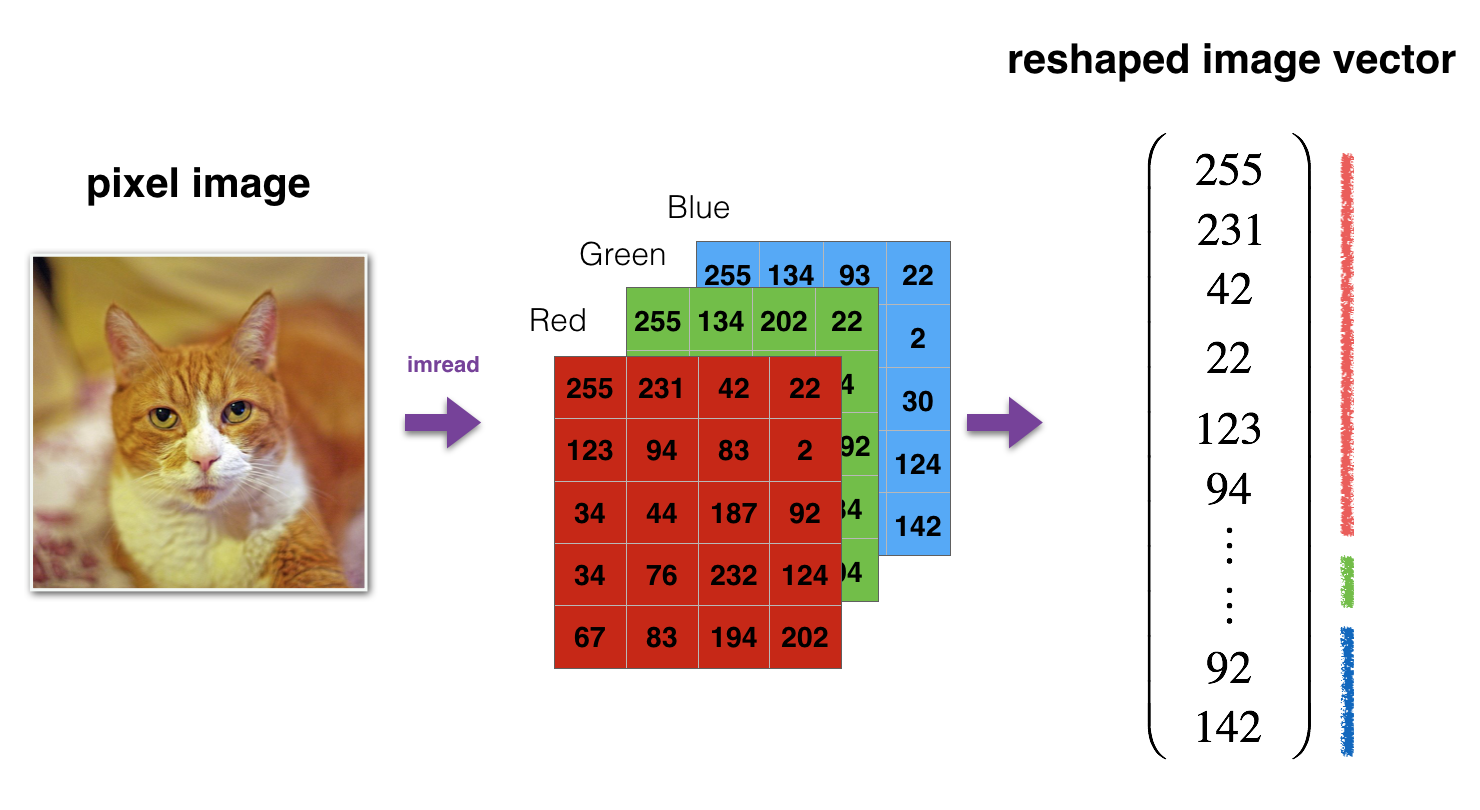
\includegraphics[width=0.9\textwidth]{course1/Image_to_vector_conversion}
\caption{Image to vector conversion}
\end{center}
\end{figure}

12288  equals 64$\times$64$\times$3 which is the size of one reshaped image vector.


\subsubsection{Architecture of your model}

Now that you are familiar with the dataset, it is time to build a deep neural network to distinguish cat images from non-cat images.

You will build two different models:
\begin{itemize}
\item A 2-layer neural network
\item An L-layer deep neural network
\end{itemize}

You will then compare the performance of these models, and also try out different values for $L$. 

Let's look at the two architectures.

\subsubsubsection{2-layer neural network}

\begin{figure}[h]
\begin{center}
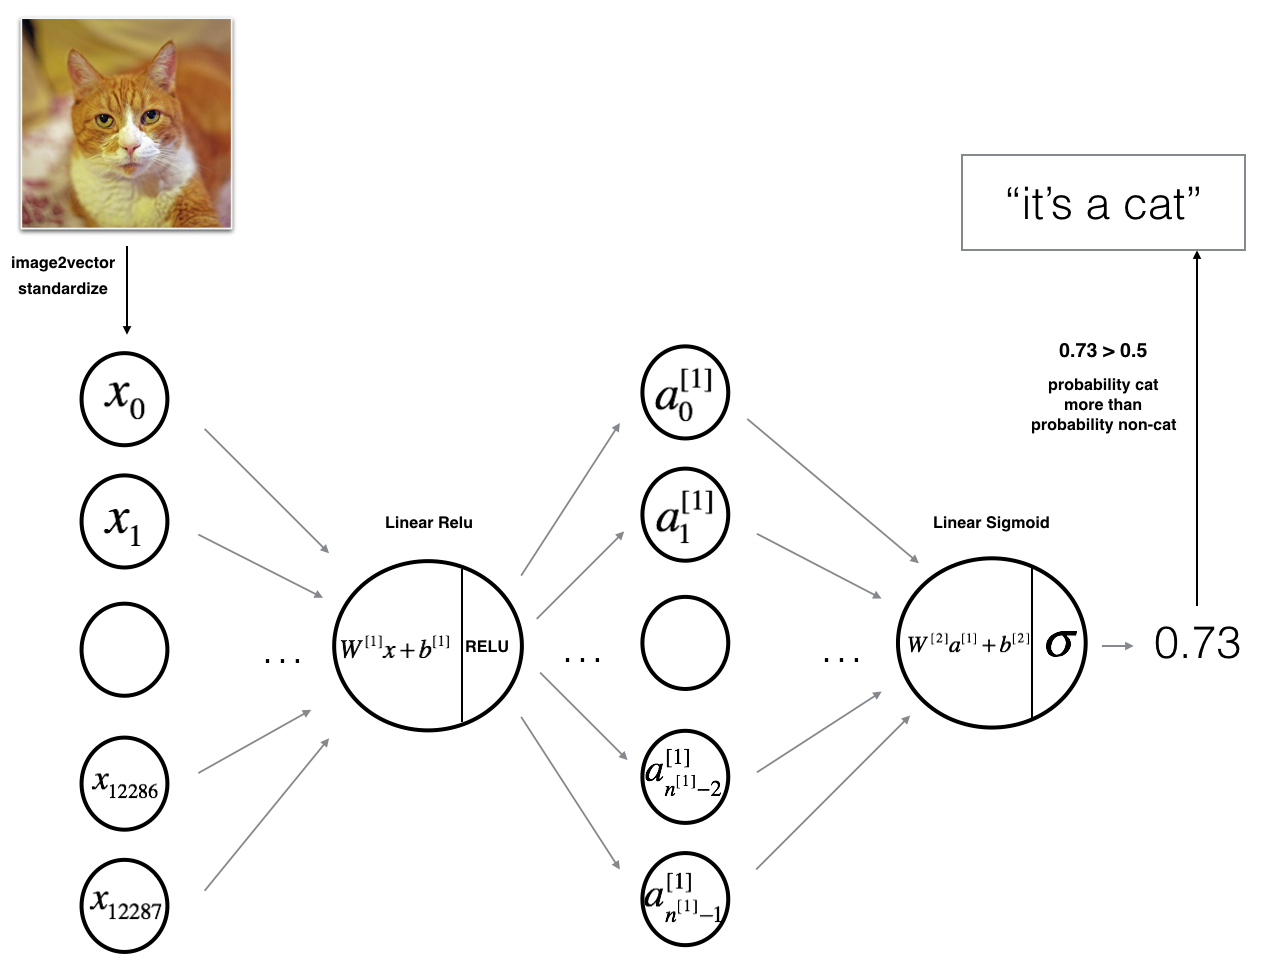
\includegraphics[width=0.65\textwidth]{course1/2layerNN}
\caption{2-layer neural network}
\label{2layerNN}
\end{center}
\end{figure}

The model can be summarized as: \emph{INPUT -> LINEAR -> RELU -> LINEAR -> SIGMOID -> OUTPUT}. Detailed Architecture of figure \ref{2layerNN}:
\begin{itemize}
\item The input is a (64,64,3) image which is flattened to a vector of size $(12288,1)$. 
\item The corresponding vector: $[x_0,x_1,...,x_{12287}]^T$ is then multiplied by the weight matrix $W^{[1]}$ of size $(n^{[1]}, 12288)$.
\item You then add a bias term and take its relu to get the following vector: $[a_0^{[1]}, a_1^{[1]},..., a_{n^{[1]}-1}^{[1]}]^T$.
\item You then repeat the same process.
\item You multiply the resulting vector by $W^{[2]}$ and add your intercept (bias). 
\item Finally, you take the sigmoid of the result. If it is greater than 0.5, you classify it to be a cat.
\end{itemize}



\subsubsubsection{L-layer deep neural network}

It is hard to represent an L-layer deep neural network with the above representation. However, figure \ref{LlayerNN} is a simplified network representation:
\begin{figure}[h]
\begin{center}
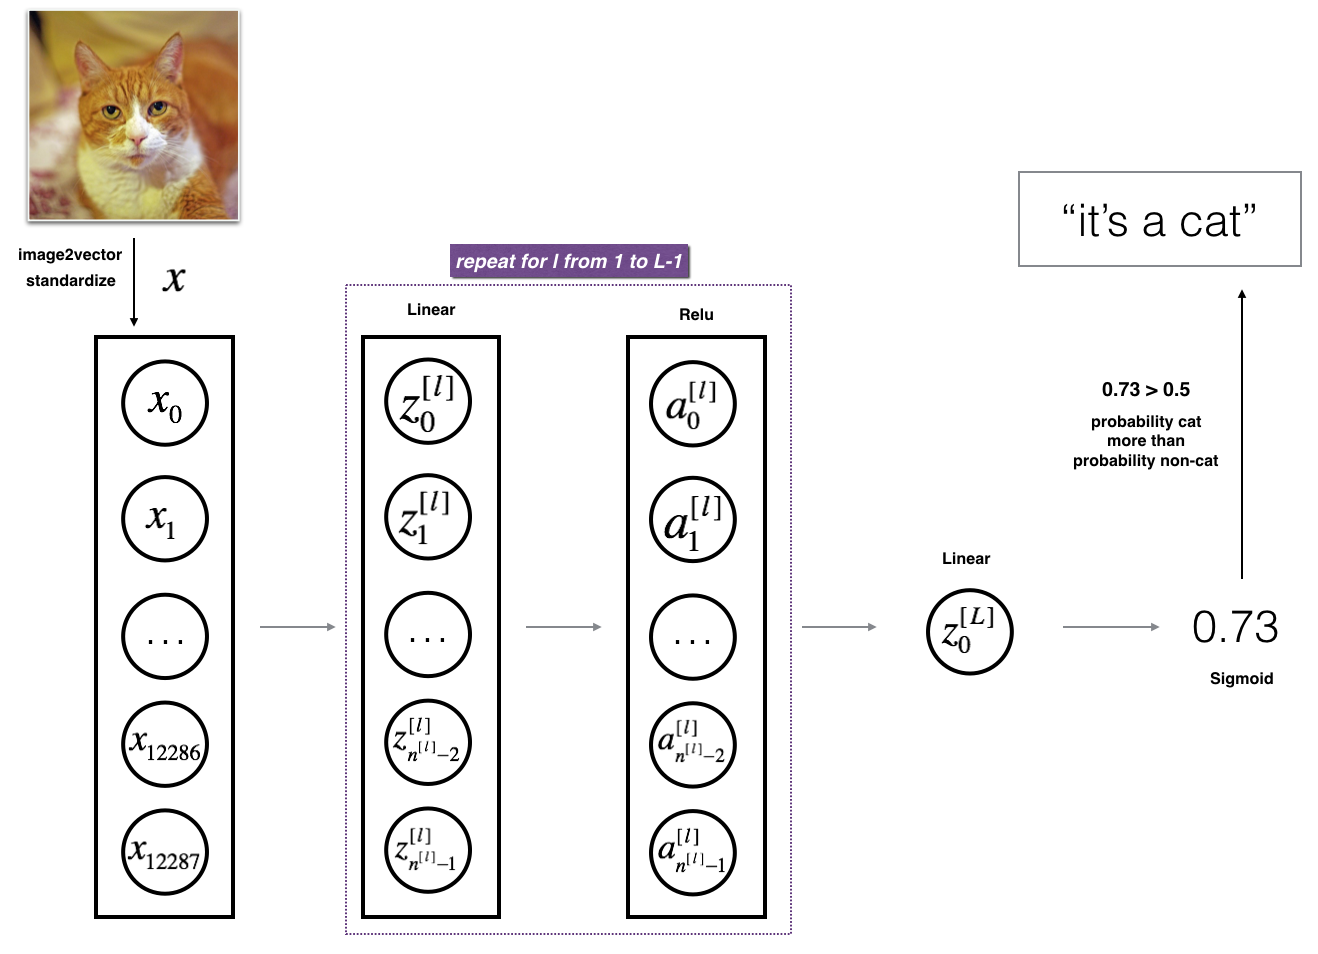
\includegraphics[width=0.65\textwidth]{course1/LlayerNN}
\caption{ L-layer neural network}
\label{LlayerNN}
\end{center}
\end{figure}


The model can be summarized as: \emph{[LINEAR -> RELU]  $\times$  (L-1) -> LINEAR -> SIGMOID}. Detailed Architecture of figure \ref{LlayerNN}:
\begin{itemize}
\item The input is a (64,64,3) image which is flattened to a vector of size (12288,1).
\item The corresponding vector: $[x_0,x_1,...,x_{12287}]^T$ is then multiplied by the weight matrix $W^{[1]}$ and then you add the intercept $b^{[1]}$. The result is called the linear unit.
\item Next, you take the relu of the linear unit. This process could be repeated several times for each $(W^{[l]}, b^{[l]})$ depending on the model architecture.
\item Finally, you take the sigmoid of the final linear unit. If it is greater than 0.5, you classify it to be a cat.
\end{itemize}



\subsubsubsection{General methodology}

As usual you will follow the Deep Learning methodology to build the model:
\begin{itemize}
\item[1.] Initialize parameters / Define hyperparameters
\item[2.] Loop for num\_iterations:
\begin{itemize}
\item[a.] Forward propagation
\item[b.] Compute cost function
\item[c.] Backward propagation
\item[d.] Update parameters (using parameters, and grads from backprop) 
\end{itemize}
\item[3.] Use trained parameters to predict labels
\end{itemize}

Let's now implement those two models!



\subsubsection{Two-layer neural network}

{\textbf {Question}}: Use the helper functions you have implemented in the previous assignment to build a 2-layer neural network with the following structure: \emph{LINEAR -> RELU -> LINEAR -> SIGMOID}. The functions you may need and their inputs are:
\begin{minted}{python}
def initialize_parameters(n_x, n_h, n_y):
    ...
    return parameters 
def linear_activation_forward(A_prev, W, b, activation):
    ...
    return A, cache
def compute_cost(AL, Y):
    ...
    return cost
def linear_activation_backward(dA, cache, activation):
    ...
    return dA_prev, dW, db
def update_parameters(parameters, grads, learning_rate):
    ...
    return parameters
\end{minted}

The whole code is as follows:

\begin{minted}{python}
### CONSTANTS DEFINING THE MODEL ####
n_x = 12288     # num_px * num_px * 3
n_h = 7
n_y = 1
layers_dims = (n_x, n_h, n_y)


# GRADED FUNCTION: two_layer_model
def two_layer_model(X, Y, layers_dims, learning_rate = 0.0075, num_iterations = 3000, print_cost=False):
    """
    Implements a two-layer neural network: LINEAR->RELU->LINEAR->SIGMOID.
    
    Arguments:
    X -- input data, of shape (n_x, number of examples)
    Y -- true "label" vector (containing 0 if cat, 1 if non-cat), of shape (1, number of examples)
    layers_dims -- dimensions of the layers (n_x, n_h, n_y)
    num_iterations -- number of iterations of the optimization loop
    learning_rate -- learning rate of the gradient descent update rule
    print_cost -- If set to True, this will print the cost every 100 iterations 
    
    Returns:
    parameters -- a dictionary containing W1, W2, b1, and b2
    """
    
    np.random.seed(1)
    grads = {}
    costs = []                              # to keep track of the cost
    m = X.shape[1]                           # number of examples
    (n_x, n_h, n_y) = layers_dims
    
    # Initialize parameters dictionary, by calling one of the functions you'd previously implemented
    ### START CODE HERE ### (≈ 1 line of code)
    parameters =initialize_parameters(n_x, n_h, n_y)
    ### END CODE HERE ###
    
    # Get W1, b1, W2 and b2 from the dictionary parameters.
    W1 = parameters["W1"]
    b1 = parameters["b1"]
    W2 = parameters["W2"]
    b2 = parameters["b2"]
    
    # Loop (gradient descent)

    for i in range(0, num_iterations):

        # Forward propagation: LINEAR -> RELU -> LINEAR -> SIGMOID. Inputs: "X, W1, b1". Output: "A1, cache1, A2, cache2".
        ### START CODE HERE ### (≈ 2 lines of code)
        A1, cache1 = linear_activation_forward(X, W1, b1, "relu")
        A2, cache2 = linear_activation_forward(A1, W2, b2, "sigmoid")
        ### END CODE HERE ###
        
        # Compute cost
        ### START CODE HERE ### (≈ 1 line of code)
        cost =  compute_cost(A2, Y)
        ### END CODE HERE ###
        
        # Initializing backward propagation
        dA2 = - (np.divide(Y, A2) - np.divide(1 - Y, 1 - A2))
        
        # Backward propagation. Inputs: "dA2, cache2, cache1". Outputs: "dA1, dW2, db2; also dA0 (not used), dW1, db1".
        ### START CODE HERE ### (≈ 2 lines of code)
        dA1, dW2, db2 = linear_activation_backward(dA2, cache2, "sigmoid")
        dA0, dW1, db1 = linear_activation_backward(dA1, cache1, "relu")
        ### END CODE HERE ###
        
        # Set grads['dWl'] to dW1, grads['db1'] to db1, grads['dW2'] to dW2, grads['db2'] to db2
        grads['dW1'] = dW1
        grads['db1'] = db1
        grads['dW2'] = dW2
        grads['db2'] = db2
        
        # Update parameters.
        ### START CODE HERE ### (approx. 1 line of code)
        parameters = update_parameters(parameters, grads, learning_rate)
        ### END CODE HERE ###

        # Retrieve W1, b1, W2, b2 from parameters
        W1 = parameters["W1"]
        b1 = parameters["b1"]
        W2 = parameters["W2"]
        b2 = parameters["b2"]
        
        # Print the cost every 100 training example
        if print_cost and i % 100 == 0:
            print("Cost after iteration {}: {}".format(i, np.squeeze(cost)))
        if print_cost and i % 100 == 0:
            costs.append(cost)
       
    # plot the cost

    plt.plot(np.squeeze(costs))
    plt.ylabel('cost')
    plt.xlabel('iterations (per tens)')
    plt.title("Learning rate =" + str(learning_rate))
    plt.show()
    
    return parameters
\end{minted}

\begin{minted}{python}
#input
parameters = two_layer_model(train_x, train_y, layers_dims = (n_x, n_h, n_y), num_iterations = 2500, print_cost=True)

#output
Cost after iteration 0: 0.693049735659989
Cost after iteration 100: 0.6464320953428849
Cost after iteration 200: 0.6325140647912678
......
Cost after iteration 2400: 0.048554785628770226
\end{minted}
\begin{figure}[h]
\begin{center}
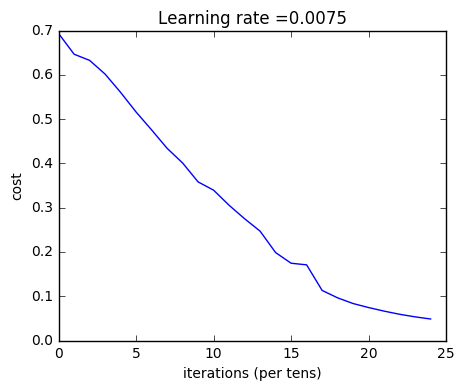
\includegraphics[width=0.6\textwidth]{course1/two_layer_model_result}
\caption{cost}
\label{two_layer_model_result}
\end{center}
\end{figure}


Now, you can use the trained parameters to classify images from the dataset. To see your predictions on the training and test sets, run the code below.
\begin{minted}{python}
predictions_train = predict(train_x, train_y, parameters)
#output
Accuracy: 1.0

predictions_test = predict(test_x, test_y, parameters)
#output
Accuracy: 0.72
\end{minted}

{\textbf {Note}}: You may notice that running the model on fewer iterations (say 1500) gives better accuracy on the test set. This is called {\color{red} \textbf {``early stopping''}} and we will talk about it in the next course. Early stopping is a way to prevent overfitting. 

Congratulations! It seems that your 2-layer neural network has better performance (72\%) than the logistic regression implementation (70\%, \hyperref[sec:logistic_regression]{assignment week 2 }). Let's see if you can do even better with an $L$-layer model.



\subsubsection{L-layer Neural Network}

{\textbf {Question}}: Use the helper functions you have implemented previously to build an $L$-layer neural network with the following structure: \emph{[LINEAR -> RELU]$\times$(L-1) -> LINEAR -> SIGMOID}. The functions you may need and their inputs are:
\begin{minted}{python}
def initialize_parameters_deep(layer_dims):
    ...
    return parameters 
def L_model_forward(X, parameters):
    ...
    return AL, caches
def compute_cost(AL, Y):
    ...
    return cost
def L_model_backward(AL, Y, caches):
    ...
    return grads
def update_parameters(parameters, grads, learning_rate):
    ...
    return parameters
\end{minted}

The whole code is as follows:
\begin{minted}{python}
### CONSTANTS ###
layers_dims = [12288, 20, 7, 5, 1] #  5-layer model

# GRADED FUNCTION: L_layer_model
def L_layer_model(X, Y, layers_dims, learning_rate = 0.0075, num_iterations = 3000, print_cost=False):#lr was 0.009
    """
    Implements a L-layer neural network: [LINEAR->RELU]*(L-1)->LINEAR->SIGMOID.
    
    Arguments:
    X -- data, numpy array of shape (number of examples, num_px * num_px * 3)
    Y -- true "label" vector (containing 0 if cat, 1 if non-cat), of shape (1, number of examples)
    layers_dims -- list containing the input size and each layer size, of length (number of layers + 1).
    learning_rate -- learning rate of the gradient descent update rule
    num_iterations -- number of iterations of the optimization loop
    print_cost -- if True, it prints the cost every 100 steps
    
    Returns:
    parameters -- parameters learnt by the model. They can then be used to predict.
    """

    np.random.seed(1)
    costs = []                         # keep track of cost
    
    # Parameters initialization.
    ### START CODE HERE ###
    parameters = initialize_parameters_deep(layers_dims)
    ### END CODE HERE ###
    
    # Loop (gradient descent)
    for i in range(0, num_iterations):

        # Forward propagation: [LINEAR -> RELU]*(L-1) -> LINEAR -> SIGMOID.
        ### START CODE HERE ### (≈ 1 line of code)
        AL, caches =  L_model_forward(X, parameters)
        ### END CODE HERE ###
        
        # Compute cost.
        ### START CODE HERE ### (≈ 1 line of code)
        cost =  compute_cost(AL, Y)
        ### END CODE HERE ###
    
        # Backward propagation.
        ### START CODE HERE ### (≈ 1 line of code)
        grads =  L_model_backward(AL, Y, caches)
        ### END CODE HERE ###
 
        # Update parameters.
        ### START CODE HERE ### (≈ 1 line of code)
        parameters =  update_parameters(parameters, grads, learning_rate)
        ### END CODE HERE ###
                
        # Print the cost every 100 training example
        if print_cost and i % 100 == 0:
            print ("Cost after iteration %i: %f" %(i, cost))
        if print_cost and i % 100 == 0:
            costs.append(cost)
            
    # plot the cost
    plt.plot(np.squeeze(costs))
    plt.ylabel('cost')
    plt.xlabel('iterations (per tens)')
    plt.title("Learning rate =" + str(learning_rate))
    plt.show()
    
    return parameters
\end{minted}


\begin{minted}{python}
#input
parameters = L_layer_model(train_x, train_y, layers_dims, num_iterations = 2500, print_cost = True)

#output
Cost after iteration 0: 0.771749
Cost after iteration 100: 0.672053
Cost after iteration 200: 0.648263
......
Cost after iteration 2400: 0.092878
\end{minted}
\begin{figure}[h]
\begin{center}
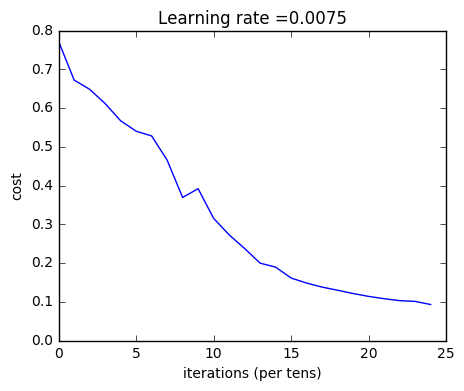
\includegraphics[width=0.6\textwidth]{course1/L_layer_model_result}
\caption{cost}
\label{L_layer_model_result}
\end{center}
\end{figure}

Now, you can use the trained parameters to classify images from the dataset. To see your predictions on the training and test sets, run the code below.
\begin{minted}{python}
pred_train = predict(train_x, train_y, parameters)
#output
Accuracy: 0.985645933014

pred_test = predict(test_x, test_y, parameters)
#output
Accuracy: 0.8
\end{minted}


Congrats! It seems that your 5-layer neural network has better performance (80\%) than your 2-layer neural network (72\%) on the same test set.

This is good performance for this task. Nice job!

Though in the next course on "Improving deep neural networks" you will learn how to obtain even higher accuracy by systematically searching for better hyperparameters (learning\_rate, layers\_dims, num\_iterations, and others you'll also learn in the next course).



\subsubsection{Results Analysis}

First, let's take a look at some images the L-layer model labeled incorrectly. This will show a few mislabeled images.
\begin{minted}{python}
print_mislabeled_images(classes, test_x, test_y, pred_test)
\end{minted}

\begin{figure}[H]
  \centering
  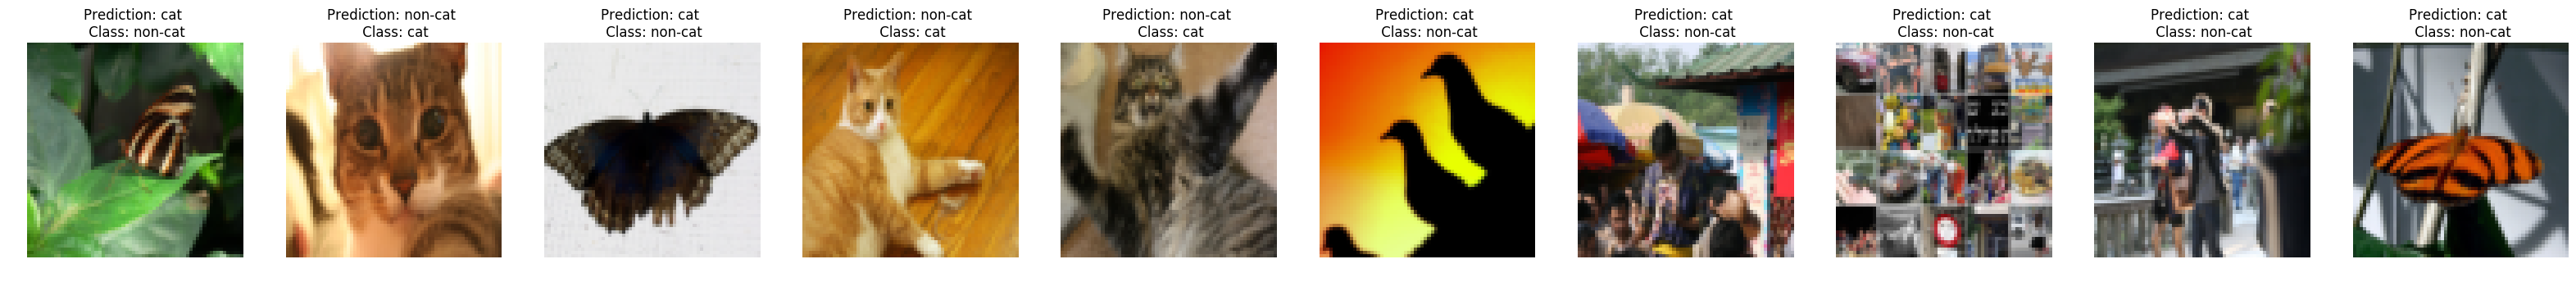
\includegraphics[width=\textwidth]{course1/mislabeled_images} 
  \caption{mislabeled images}
\end{figure}

{\textbf {A few type of images the model tends to do poorly on include}}:
\begin{itemize}
\item Cat body in an unusual position
\item Cat appears against a background of a similar color
\item Unusual cat color and species
\item Camera Angle
\item Brightness of the picture
\item Scale variation (cat is very large or small in image)
\end{itemize}



\subsubsection{Test with your own image (optional/ungraded exercise)}

Congratulations on finishing this assignment. You can use your own image and see the output of your model. To do that:
\begin{itemize}
\item[1.] Click on ``File'' in the upper bar of this notebook, then click ``Open'' to go on your Coursera Hub.
\item[2.] Add your image to this Jupyter Notebook's directory, in the ``images'' folder
\item[3.] Change your image's name in the following code
\item[4.] Run the code and check if the algorithm is right (1 = cat, 0 = non-cat)!
\end{itemize}

\begin{minted}{python}
## START CODE HERE ##
my_image = "test_cat3.jpg" # change this to the name of your image file 
my_label_y = [1] # the true class of your image (1 -> cat, 0 -> non-cat)
## END CODE HERE ##

fname = "images/" + my_image
image = np.array(ndimage.imread(fname, flatten=False))
my_image = scipy.misc.imresize(image, size=(num_px,num_px)).reshape((num_px*num_px*3,1))
my_predicted_image = predict(my_image, my_label_y, parameters)

plt.imshow(image)
print ("y = " + str(np.squeeze(my_predicted_image)) + ", your L-layer model predicts a \"" + classes[int(np.squeeze(my_predicted_image)),].decode("utf-8") +  "\" picture.")


#output:
Accuracy: 1.0
y = 1.0, your L-layer model predicts a "ca" picture.
\end{minted}

\begin{figure}[H]
  \centering
  
\includegraphics[width=0.6\textwidth]{course1/test_cat3} 
\end{figure}

\clearpage
\subsubsection{Code of Deep Neural Network for Image Classification: Application}
\begin{minted}{python}
#matplotlib inline
plt.rcParams['figure.figsize'] = (5.0, 4.0) # set default size of plots
plt.rcParams['image.interpolation'] = 'nearest'
plt.rcParams['image.cmap'] = 'gray'

np.random.seed(1)

#Load the data 
train_x_orig, train_y, test_x_orig, test_y, classes = load_data()

#=====================================================
# #show an image in the dataset. Example of a picture
# index = 12
# plt.imshow(train_x_orig[index])
# print ("y = " + str(train_y[0,index]) + ". It's a " + classes[train_y[0,index]].decode("utf-8") +  " picture.")
#=====================================================

# Explore your dataset 
m_train = train_x_orig.shape[0]
m_test =  test_x_orig.shape[0]
num_px = train_x_orig.shape[1]

# Reshape the training and test examples 
train_x_flatten = train_x_orig.reshape(train_x_orig.shape[0], -1).T   # The "-1" makes reshape flatten the remaining dimensions
test_x_flatten = test_x_orig.reshape(test_x_orig.shape[0], -1).T

# Standardize data to have feature values between 0 and 1.
train_x = train_x_flatten/255.
test_x = test_x_flatten/255.


### CONSTANTS DEFINING THE MODEL ####
n_x = 12288     # num_px * num_px * 3
n_h = 7
n_y = 1
layers_dims = (n_x, n_h, n_y)


# GRADED FUNCTION: two_layer_model

def two_layer_model(X, Y, layers_dims, learning_rate = 0.0075, num_iterations = 3000, print_cost=False):
    """
    Implements a two-layer neural network: LINEAR->RELU->LINEAR->SIGMOID.
    
    Arguments:
    X -- input data, of shape (n_x, number of examples)
    Y -- true "label" vector (containing 0 if cat, 1 if non-cat), of shape (1, number of examples)
    layers_dims -- dimensions of the layers (n_x, n_h, n_y)
    num_iterations -- number of iterations of the optimization loop
    learning_rate -- learning rate of the gradient descent update rule
    print_cost -- If set to True, this will print the cost every 100 iterations 
    
    Returns:
    parameters -- a dictionary containing W1, W2, b1, and b2
    """
    
    np.random.seed(1)
    grads = {}
    costs = []                              # to keep track of the cost
    m = X.shape[1]                           # number of examples
    (n_x, n_h, n_y) = layers_dims
    
    # Initialize parameters dictionary, by calling one of the functions you'd previously implemented
    parameters =initialize_parameters(n_x, n_h, n_y)
    
    # Get W1, b1, W2 and b2 from the dictionary parameters.
    W1 = parameters["W1"]
    b1 = parameters["b1"]
    W2 = parameters["W2"]
    b2 = parameters["b2"]
    
    # Loop (gradient descent)
    for i in range(0, num_iterations):
        # Forward propagation: LINEAR -> RELU -> LINEAR -> SIGMOID. Inputs: "X, W1, b1". Output: "A1, cache1, A2, cache2".
        A1, cache1 = linear_activation_forward(X, W1, b1, "relu")
        A2, cache2 = linear_activation_forward(A1, W2, b2, "sigmoid")
        
        # Compute cost
        cost =  compute_cost(A2, Y)
        
        # Initializing backward propagation
        dA2 = - (np.divide(Y, A2) - np.divide(1 - Y, 1 - A2))
        
        # Backward propagation. Inputs: "dA2, cache2, cache1". Outputs: "dA1, dW2, db2; also dA0 (not used), dW1, db1".
        dA1, dW2, db2 = linear_activation_backward(dA2, cache2, "sigmoid")
        dA0, dW1, db1 = linear_activation_backward(dA1, cache1, "relu")
        
        # Set grads['dWl'] to dW1, grads['db1'] to db1, grads['dW2'] to dW2, grads['db2'] to db2
        grads['dW1'] = dW1
        grads['db1'] = db1
        grads['dW2'] = dW2
        grads['db2'] = db2
        
        # Update parameters.
        parameters = update_parameters(parameters, grads, learning_rate)

        # Retrieve W1, b1, W2, b2 from parameters
        W1 = parameters["W1"]
        b1 = parameters["b1"]
        W2 = parameters["W2"]
        b2 = parameters["b2"]
        
        # Print the cost every 100 training example
        if print_cost and i % 100 == 0:
            print("Cost after iteration {}: {}".format(i, np.squeeze(cost)))
        if print_cost and i % 100 == 0:
            costs.append(cost)
       
    # plot the cost
    plt.plot(np.squeeze(costs))
    plt.ylabel('cost')
    plt.xlabel('iterations (per tens)')
    plt.title("Learning rate =" + str(learning_rate))
    plt.show()
    
    return parameters



# GRADED FUNCTION: L_layer_model
def L_layer_model(X, Y, layers_dims, learning_rate = 0.0075, num_iterations = 3000, print_cost=False):#lr was 0.009
    """
    Implements a L-layer neural network: [LINEAR->RELU]*(L-1)->LINEAR->SIGMOID.
    
    Arguments:
    X -- data, numpy array of shape (number of examples, num_px * num_px * 3)
    Y -- true "label" vector (containing 0 if cat, 1 if non-cat), of shape (1, number of examples)
    layers_dims -- list containing the input size and each layer size, of length (number of layers + 1).
    learning_rate -- learning rate of the gradient descent update rule
    num_iterations -- number of iterations of the optimization loop
    print_cost -- if True, it prints the cost every 100 steps
    
    Returns:
    parameters -- parameters learnt by the model. They can then be used to predict.
    """

    np.random.seed(1)
    costs = []                         # keep track of cost
    
    # Parameters initialization.
    parameters = initialize_parameters_deep(layers_dims)
    
    # Loop (gradient descent)
    for i in range(0, num_iterations):

        # Forward propagation: [LINEAR -> RELU]*(L-1) -> LINEAR -> SIGMOID.
        AL, caches =  L_model_forward(X, parameters)
        
        # Compute cost.
        cost =  compute_cost(AL, Y)
    
        # Backward propagation.
        grads =  L_model_backward(AL, Y, caches)
 
        # Update parameters.
        parameters =  update_parameters(parameters, grads, learning_rate)
                
        # Print the cost every 100 training example
        if print_cost and i % 100 == 0:
            print ("Cost after iteration %i: %f" %(i, cost))
        if print_cost and i % 100 == 0:
            costs.append(cost)
            
    # plot the cost
    plt.plot(np.squeeze(costs))
    plt.ylabel('cost')
    plt.xlabel('iterations (per tens)')
    plt.title("Learning rate =" + str(learning_rate))
    plt.show()
    
    return parameters

### CONSTANTS ###
layers_dims = [12288, 20, 7, 5, 1] #  5-layer model

# two_layer_model
parameters_two_layer_model = two_layer_model(train_x, train_y, layers_dims = (n_x, n_h, n_y), num_iterations = 2500, print_cost=True)
predictions_train = predict(train_x, train_y, parameters_two_layer_model)
predictions_test = predict(test_x, test_y, parameters_two_layer_model)


# L_layer_model
parameters_L_layer_model = L_layer_model(train_x, train_y, layers_dims, num_iterations = 2500, print_cost = True)
pred_train = predict(train_x, train_y, parameters_L_layer_model)
pred_test = predict(test_x, test_y, parameters_L_layer_model)
\end{minted}
\clearpage